
\chapter{Hardware Injection through Photon Calibrator}
\section{Principle}



 
 As I described in Sec.\ref{sec:pcalth}, we can generate desired ETM displacement $x(t)$ by changing PCal laser intensity $P(t)$. One can calculate corresponding $P(t)$ by performing inverse Fourier transform to Eq.(\ref{eq:pcaldisp}).
 
\begin{align}
    \int_{-\infty}^{-\infty} x(\omega) e^{i \omega t} ~\mathrm{d} \omega &= 
     \frac{-2   \cos(\theta)}{Mc} 
     \int_{-\infty}^{-\infty}\frac{P(\omega)}{\omega^2} e^{i \omega t} ~\mathrm{d} \omega \\
\label{eq:pcaldispt}
    \frac{Mc}{-2 \cos(\theta)} \int_{-\infty}^{-\infty}
     x(\omega) \omega^2 e^{i \omega t} ~\mathrm{d} \omega 
&= P(t) 
\end{align}

where
\begin{align*}
%\label{eq:pcaleq}
   \text{Mass of ETM} \qquad  M &= 23 ~\mathrm{kg} \\
   \text{Arm Length} \qquad   L &= 3 ~\mathrm{km}  \\
   \text{Angle of Incident} \qquad   \theta &= 0.72 ~\mathrm{deg}  \\
   \text{Speed of Light} \qquad   c &= 2.998\times10^8 ~\mathrm{m/s} \\
\end{align*}
Also, if we have complete suspension model of ETM, we can substitute the $\omega^2$ factor in Eq.(\ref{eq:pcaldispt}) by the full displacement-to-force transfer function.

Once we got the necessary P(t) from the desired x(t) through Eq.(\ref{eq:pcaldispt}), we can start to modulate our PCal laser intensity according to that P(t). The way how we control our PCal laser intensity is explained in Fig.~(\ref{fig:injsigpath}).


\begin{figure}[hbt!]
\centering
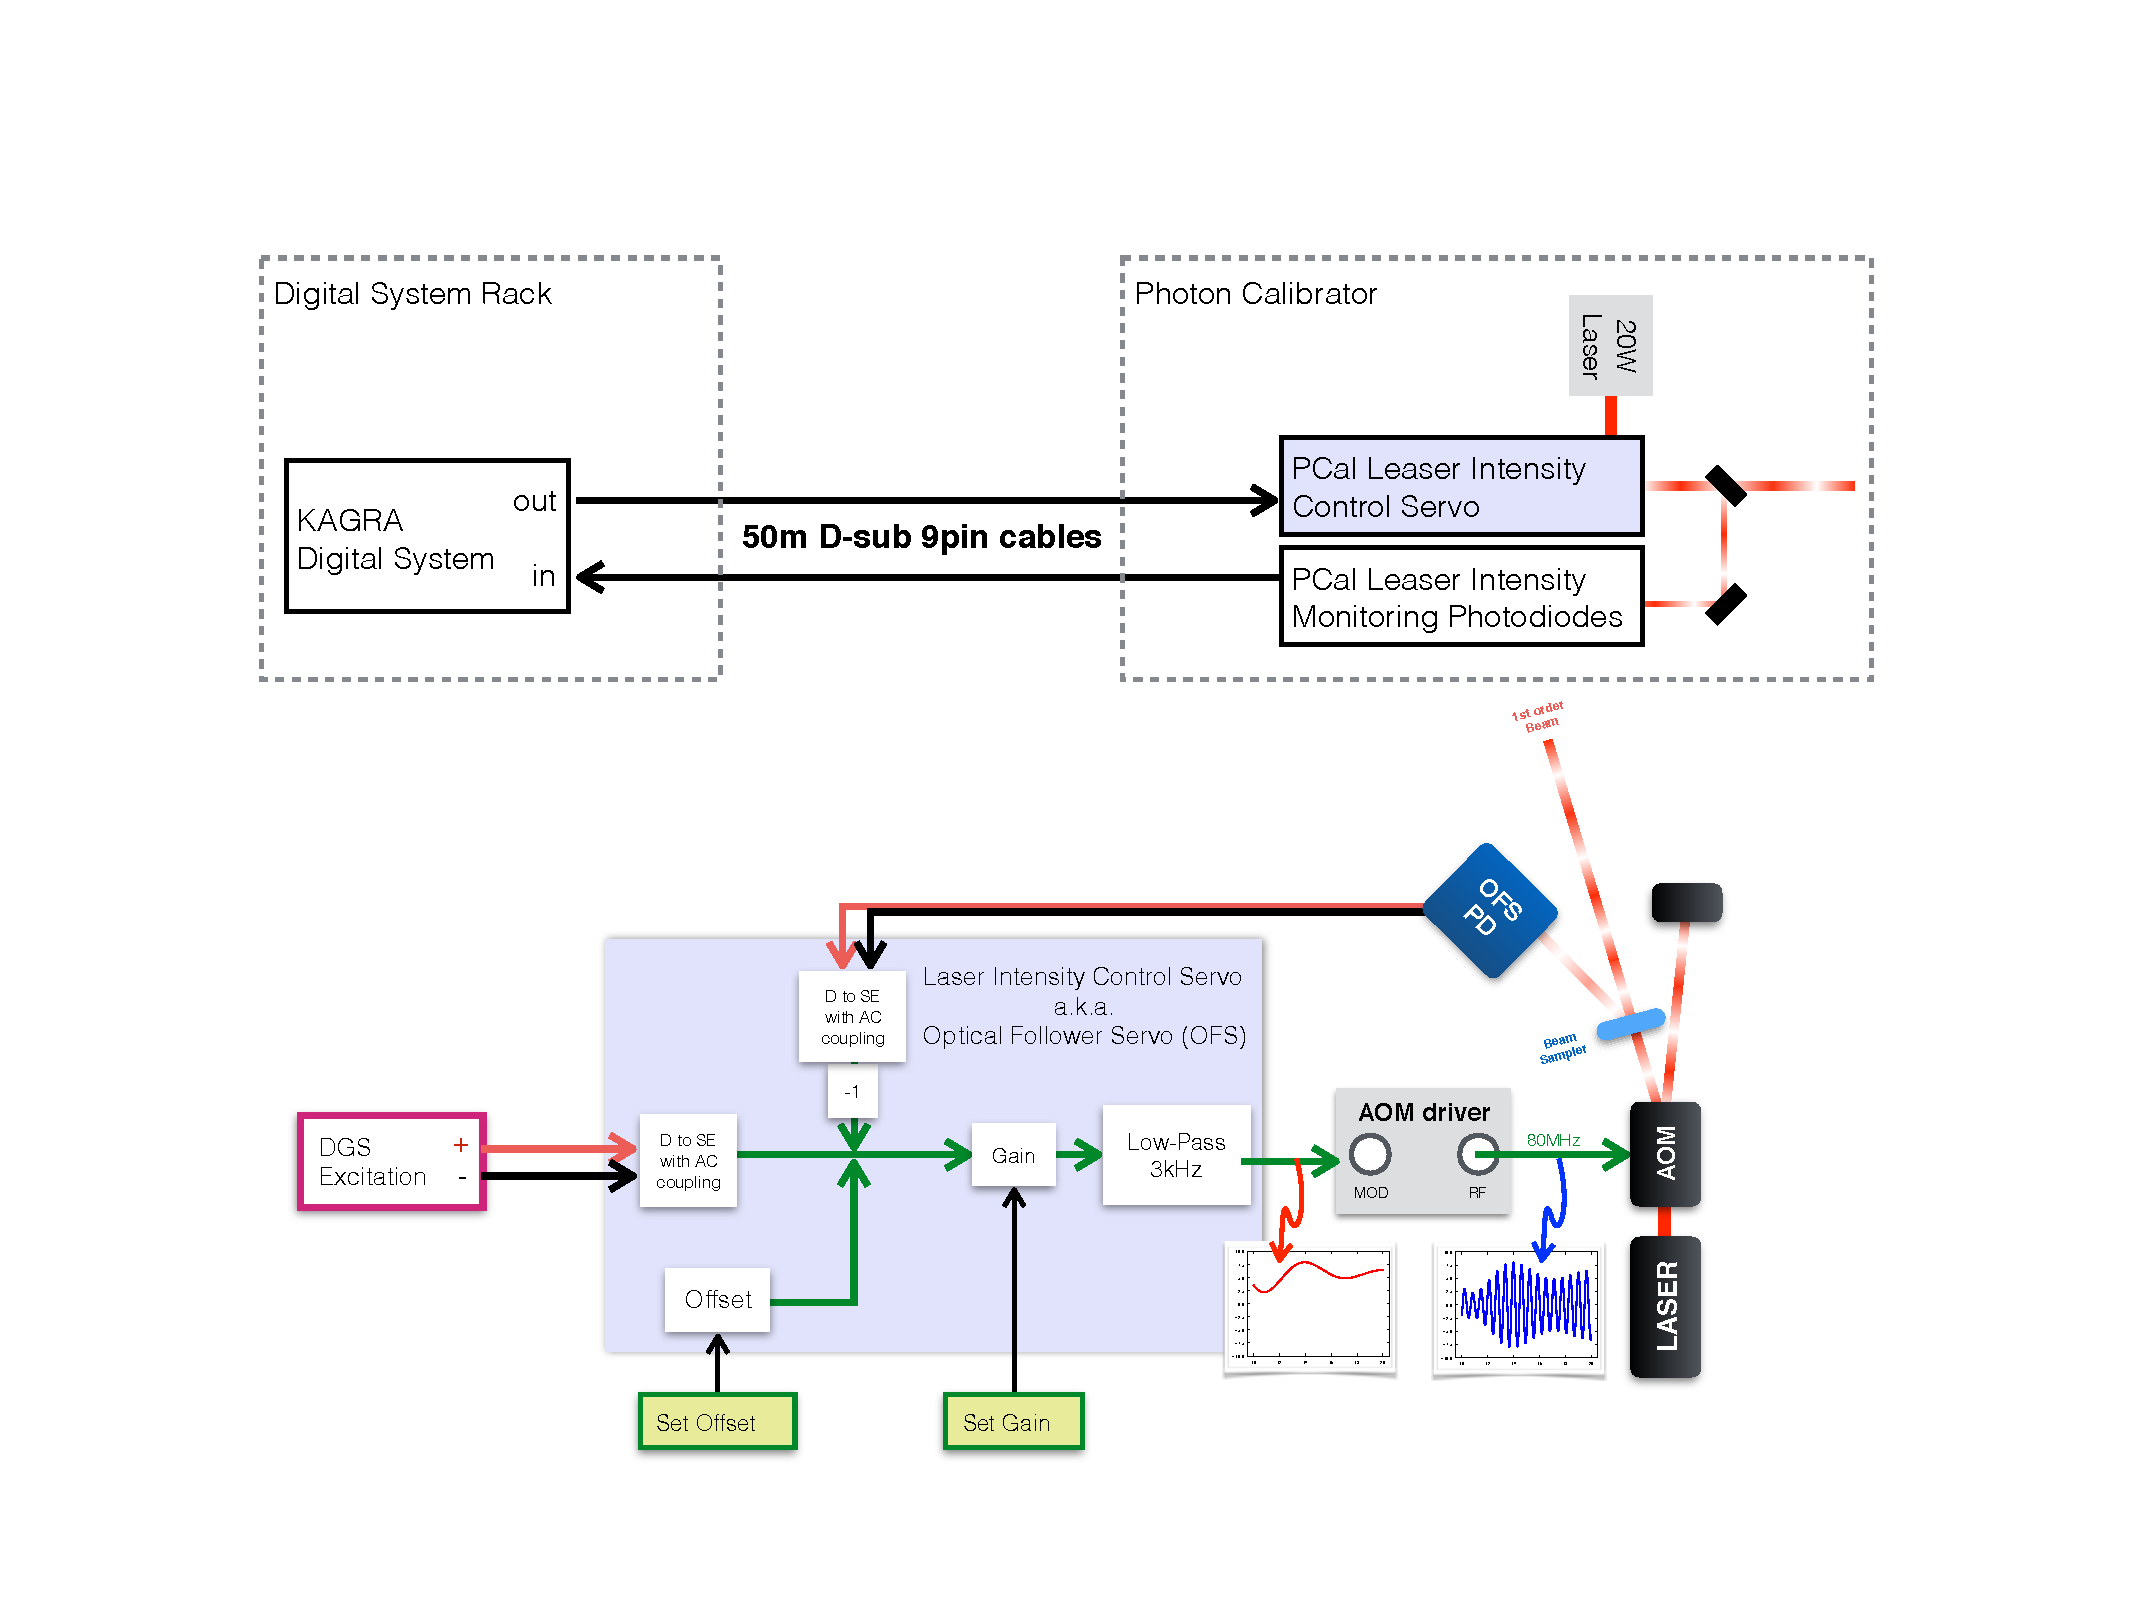
\includegraphics[width=1\textwidth]{figure/injsigpath}
\caption[Controlling PCal with Digital Control System]{Controlling PCal with Digital Control System. The PCal laser beam that will be sent to ETM is the first order diffracted beam of a 20W input laser form an acousto-optic modulator(AOM). Its intensity is controlled by the control signal from our KAGRA Digital System. An analog feedback control loop called Optical Follower Servo(OFS) has been implemented to reduce non-linear response of AOM and laser intensity noise of 20W input laser.  }
\label{fig:injsigpath}
\index{figures}
\end{figure}


%
%Validate IFO by Pcal (Hardware Injection Test)
%As I mentioned in last chapter, the practical response of IFO is very complex. To prevent some unexpected problem including no-linear response of IFO and……  
%The best way is to provide some test source of expected GW signal.
%
%However, it is almost impossible to prepare, for example, a binary blackhole system in laboratory. Instead, we will generated some test signal by pushing the ETM with Pcal. This procedure is called “Hardware Injection Test”
%
%
%Motivation
%To under whether we can successfully reconstruct the h(t) from our interferometer, the best way is to prepare an artificial signal, sending it to interferometer, reconstructing it, finally, comparing it with original one. However it is quite difficult to generate human made gravitational wave that can be detected by current gravitational wave detector.
%
%Requirement
%
%Low Frequency
%around 100Hz  the nose should below the IFO sensitivity
%(absolute timing < ?us ns )
%
%High Frequency
%above 1kHz    the transfer function should as flat as possible


%\subsubsection{Amplitude of Injection Signal}

%\begin{equation}
%\label{eq:pcaleq}
%    \Delta L (f) (\mathrm{m} / \mathrm{Hz}) = \frac{2 \Delta P \cos(\theta)}{c} \frac{1}{M (2 \pi f )^2}
%\end{equation}
%
%\begin{align}
%%\label{eq:pcaleq}
%    \frac{F(t)}{M}=\frac{1}{M} \frac{2 P(t) \cos(\theta)}{c} &= \ddot{x}(t)
%\end{align}
%
%For $x=x_0 \sin(\omega t)$,
%\begin{align}
%%\label{eq:pcaleq}
%    \frac{1}{M} \frac{2 P_0 \cos(\theta)}{c} \sin(\omega t) &=  -\omega^2 x_0 \sin(\omega t)
%\end{align}
%
%Thus,
%\begin{align}
%%\label{eq:pcaleq}
%    P_0 &= -\omega^2 \frac{M c}{2 \cos(\theta)} x_0 = -\omega^2 \frac{M c}{2 \cos(\theta)} L h_0
%\end{align}







%\begin{align*}
%%\label{eq:pcaleq}
%    P_0 ~(\mathrm{Watts}) \times \frac{Gain_{\text{~Power to OFSPD}}}{2} &= 
%     \underbrace{V_{\text{OFSPD}}}_{\text{Same as V$_{\text{Injection}}$}}~ (\mathrm{Volts}) \\
%\end{align*}
%Therefore, the overall gain should be set in injection channel, which is in Volt unit, is
%\begin{align}
%%\label{eq:pcaleq}
%    \omega^2 \frac{M c}{2 \cos(\theta)} L \times \frac{Gain_{\text{~Power to OFSPD}} }{2}
%\end{align}

